\chapter{Reinforcement learning}\label{chap:Reinforcement Learning}

\section{Introduction}\label{sec:RL-introduction}
\ac{RL} was inspired by human and animal learning \cite{SuttonBarto:98}. It is derived from the idea that behavior can be learned by receiving rewards or punishments for good or bad actions. The result of random actions in different situations is used to decide on actions in future situations that are similar. \ac{RL} has a distinct 'trial and error' nature. Random actions are being tried until the best action for a certain situation is found. In this chapter we introduce the \ac{RL} framework and introduce various ways in which a \ac{RL} problem can be solved. After a general overview of the \ac{RL} method, we give a formal description of the framework. Finally, several solution methods are introduced and some interesting research possibilities are indicated.

In \ac{RL}, learning is done by an \emph{agent} in close interaction with its \emph{environment} (\figref{fig:RL-RLframework}). The agent is the `learner' and the `decision maker'. It decides on what \emph{action} to take and evaluates the result of this action. The agent interacts with the environment and receives feedback in the form of a scalar \emph{reward} that indicates how 'good' the previous action was. In control applications, the agent will be represented by a computer program following a certain learning algorithm and the environment will be a system (either a real setup or a mathematical model) that reacts to the actions the agents takes. The environment also gives a reward signal to the agent. We are focusing on control applications, so we assume that the decisions of the agent take place at discrete time intervals. 
\begin{figure}[htbp]
	\centering
%		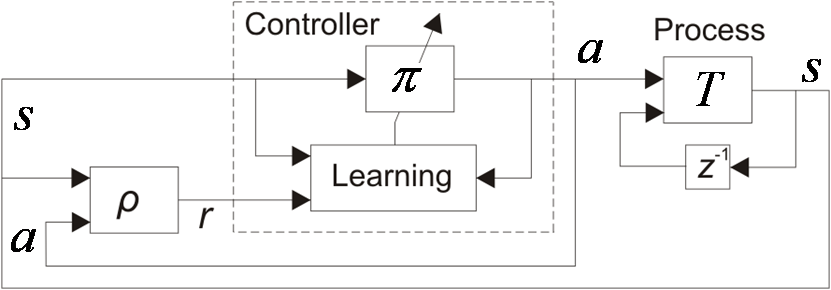
\includegraphics[width=.5\textwidth]{img/RLframework}
		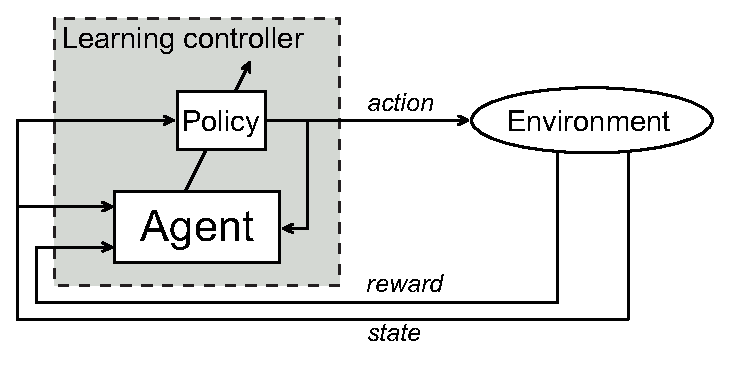
\includegraphics[width=.5\textwidth]{img/RLoverview}
	\caption[Overview of the \acs{RL} framework]{A schematic overview of the \ac{RL} framework. The agent interacts with an environment and learns using a scalar reward.}
	\label{fig:RL-RLframework}
\end{figure}

In many problems, a certain \emph{goal} state exists that the agent must try to reach. If this goal state is reached, the learning is stopped and the process is repeated. These separate experiments are called \emph{episodes} or \emph{trials}. The reward function can be defined in a number of ways. Usually, the reward will be positive if the goal is reached and negative or zero in all other cases. Note that the reward only qualifies the direct result of a certain action and not the long-term effects of that action. The task of the agent will be to maximize the total (accumulated) reward, which requires the agent to asses the long-term effects of actions.

After a learning process, the agent `knows' how it can reach the goal. To be more precise, it knows what action it must take in every state in order to maximize the total reward. The set of rules that describe what action the agent will take in every state is called the \emph{policy}.

So, in summary, the goal of a \ac{RL} system is to find an optimal policy so that the total reward received during a trial is maximized. This is learned by an agent in close interaction with its environment. 

\section{MDP framework}\label{sec:RL-MDP_framework}
In the previous section we introduced the general idea behind \ac{RL} and some important terms used in \ac{RL}. In this section, a more formal description of a \ac{RL} problem will be given.

A requirement in \ac{RL} is that the environment should have the Markov property. This means that if the current state is known, then the transition to the next state is independent of all previous states. However, this transition may still be either deterministic or stochastic. The state therefore contains all the information that describes the environment. In every state the agent has to make a decision based on an environment that has the Markov property, the learning task is therefore called a \ac{MDP}. When the state is only partially observable for the agent, such a task is called a \ac{POMDP}. In this work we only consider situations in which the full state is available to the agent.

Formally a \ac{MDP} is a 4-tuple $(\mathcal{S},\mathcal{A},T,\rho)$. \lsymb{$\mathcal{S}$}{Set of states} is a finite set of states \lsymb{$s$}{Single state} and \lsymb{$\mathcal{A}$}{Set of actions} a finite set of actions \lsymb{$a$}{Single action}. $\lsymb{T}{Transition function}:\mathcal{S}\times \mathcal{A}\times \mathcal{S} \rightarrow [0,1]$ is the state transition function which defines the probability of getting from state $s$ to $s'$ when action $a$ is taken. \gsymb{$\rho$}{Reward function}$:\mathcal{S}\times \mathcal{A}\times \mathcal{S} \rightarrow  \mathbb{R}$ defines the immediate reward \lsymb{$r$}{Immediate reward} for getting from state $s$ to $s'$ after taking action $a$. 

The policy is a mapping \gsymb{$\pi$}{Policy}$ : \mathcal{S} \rightarrow \mathcal{A}$ that assigns action selection probabilities to $\forall a \in \mathcal{A}$ in each state. The objective of the agent is to learn a policy that maximizes the expected total reward in the entire episode. The accumulated total reward is called the return. The expected return \lsymb{$R_t$}{Return} after an action at time step \lsymb{$t$}{Time} is:
$$%\begin{equation}\label{eqn:RL-totalReward} 
	R_t = E\left\{ r_{t+1} + \gamma r_{t+2} + \gamma^2 r_{t+3} + ...\right\} = E\left\{ \sum_{t=0}^\infty\gamma^t r_{t+1} \right\}  
$$%\end{equation}
where $\gamma\in (0,1]$ is the discount factor. In other words, $R_t$ is the sum of the expected reward for the current action and the discounted rewards of future actions when using the current policy. For problems with a finite time horizon, the upper bound of the summation is the final time step $t_\mathrm{f}$. The discount factor can be viewed in two different ways. The first view is purely mathematical. It makes sure that if the time horizon is infinite, the total reward converges to some finite value and will not go to infinity. The second view is more intuitive. By using a discount factor, rewards in the near future have an exponentially greater effect than rewards received in the far future. Because the discount factor is part of the learning task, the \ac{MDP} is sometimes explicitly written as $(\mathcal{S},\mathcal{A},T,\rho,\gamma)$ to emphasize the discounting. 

\subsection{Value functions}\label{sec:RL-Value_functions}
We can now proceed to assign a value to every state. The value of a state \lsymb{$V(s)$}{Value function} is the expected total reward in that state under a certain policy. This value function is therefore defined as:
$$%\begin{equation}\label{eqn:RL-valueFunctionDefinition} 
	V^\pi(s)=E^\pi \left\{ R_t \mid s_t=s  \right\}
$$%\end{equation}
where $E^\pi\{\cdot\}$ is the expected value when following policy $\pi$. Because the goal of the agent is to learn which action is best in every state, it is also useful to define a value function that assigns a value to state-action pairs. To this end, the action-value function \lsymb{$Q(s,a)$}{Action-value function} is defined:
$$%\begin{equation}\label{eqn:RL-actionValueFunctionDefinition} 
	Q^\pi(s,a)=E^\pi \left\{ R_t \mid s_t=s,a_t=a \right\}
$$%\end{equation}
which also depends on the policy followed. Typically, for problems in which the agent knows how it can reach a certain state, the value function $V(s)$ is convenient to use. For problems in which the agent does not know this, the action-value function $Q(s,a)$ can be used to explicitly store the reward for certain actions. In most control problems the action-value function is used.



\subsection{Optimal policy}\label{sec:RL-Optimal_policy}
As mentioned before, the goal of the agent is to take actions which will result in the highest return $R$. In other words, it has to find a policy $\pi$ that maximizes the value function $V^\pi(s)$ (or equivalently, $Q^\pi(s,a)$). This policy, which is better than all other policies, is called an optimal policy \gsymb{$\pi^*$}{Optimal policy}. The value function that belongs to this policy is the optimal value function $V^*(s)$ and is defined as:
\begin{equation}\label{eqn:RL-optimalValueFunction}
	V^*=\max_{\pi} V^\pi(s)
\end{equation}
An optimal policy has an optimal action-value function $Q^*(s,a)$:
\begin{equation}\label{eqn:RL-optimalActionValueFunction} 
	Q^*(s,a) = \max_{\pi} Q^\pi(s,a) 
\end{equation}
which can also be written in terms of the optimal value function:
$$%\begin{equation}
	Q^*(s,a) = E \left\{ r_{t+1} + \gamma V^* (s_{t+1}) \mid s_t=s,a_t=a \right\} 
$$%\end{equation}
So, if the optimal (action-)value function is known, the optimal policy is the argument that maximizes \eqref{eqn:RL-optimalValueFunction} or \eqref{eqn:RL-optimalActionValueFunction}:
$$%\begin{equation}\label{eqn:RL-optimalPolicy}
	\pi^* = \arg\max_a Q^*(s,a) = \arg\max_a E \left\{ r_{t+1} + \gamma V^* (s_{t+1}) \mid s_t=s,a_t=a \right\} 
$$%\end{equation}
Because this policy selects the action for which the (action-)value function is maximum, this policy is called a greedy policy.

Important for a large number of solution techniques are the so called Bellman equations. For the value function, these can be written as:
$$%\begin{equation}\label{eqn:RL-bellmanEquations}
	\begin{aligned}
		V^\pi(s) &= E^\pi \left\{ \sum_{t=0}^{\infty}\gamma^t r_{t+1} \mid s_t=s \right\} \\
		& = E^\pi \left\{ r_{t+1} + \gamma\sum_{t=0}^{\infty}\gamma^t r_{t+2} \mid s_t = s \right\} \\
		& = E^\pi \left\{ r_{t+1} + \gamma V^\pi(s') \mid s_t = s, s_{t+1} = s' \right\} \\
		& = \sum_{s'} T(s,a,s') \left[ \rho(s,a,s') +\gamma V^\pi(s') \right]
	\end{aligned}
$$%\end{equation}
Recall that $T(s,a,s')$ is the transition probability from $s$ to $s'$ under action $a$ and $\rho(s,a,s')$ is the scalar reward for that transition. Using \eqnref{eqn:RL-optimalValueFunction} we can derive the Bellman optimality equation for the value function:
\begin{equation}\label{eqn:RL-bellmanOptimalityEquationStateValues}
	V^*(s) = \max_{a} \sum_{s'} T(s,a,s') \left[ \rho(s,a,s') +\gamma V^\pi(s') \right]
\end{equation}
and the equivalent Bellman optimality equation for the action-value function:
\begin{equation}\label{eqn:RL-bellmanOptimalityEquationActionStateValues}
	Q^*(s) = \sum_{s'} T(s,a,s') \left[ \rho(s,a,s') +\gamma \max_{a'}Q^*(s',a') \right]
\end{equation}


\section{Solution methods}\label{sec:RL-Solution_methods}
Several methods for solving \ac{RL} problems exist. 'Solving' in a RL context means computing the optimal policy, which is generally derived from the optimal (action-)value function. The methods can be divided into three different types: model-based, model-free and model-learning methods. Model-based methods assume that a complete model of the environment is available. Model-free methods start with no knowledge of the environment at all and learn from interaction with the environment. Model-learning methods build a model during the learning process. Although prior knowledge of the environment can be incorporated, the main feature of this method is the continuous improvement of the model during learning.

\subsection{Model-based methods}\label{sec:RL-Model_based_methods}
Model-based RL methods assume that the \ac{MDP} is completely known and available to the agent. Not only is the state fully observable by the agent, also the state transition function $T$ and reward function $\rho$ are known. This means that the agent has a perfect and complete model of the environment and its dynamics. The agent can calculate for every state the possible next states and their rewards. The Bellman optimality equations \eqnref{eqn:RL-bellmanOptimalityEquationStateValues} and \eqnref{eqn:RL-bellmanOptimalityEquationActionStateValues} lead to a system of equations with only $V^*(s)$ and $Q^*(s,a)$ as unknown variables and can therefore be solved. The need for a perfect model and the computational effort needed to solve these equations, makes the practical usability for these methods limited. However, these algorithms form the base of other methods. These model-based solution techniques are called \ac{DP} \cite{Bellman:57}. We will briefly describe the Q-iteration method.
			
\subsubsection{Q-iteration}\label{sec:RL-Q_iteration}
%Q-iteration is a model-based method that 

For control applications, using the action-value function $Q(s,a)$ is usually preferred over the value function $V(s)$. Q-iteration is a model-based solution method that iteratively computes the optimal action-value function $Q^*(s,a)$. The algorithm continuously visits all state-action pairs $(s,a)$ and updates the value of $Q(s,a)$ according to the reward. The Q-iteration method is shown in Algorithm \ref{alg:Q-iteration}. For discrete state-action spaces the algorithm will always converge to the optimal policy. 

\begin{algorithm}[ht]
	\caption{Q-iteration} \label{alg:Q-iteration}
	\begin{algorithmic}[1]
		\State Initialize $Q_0(s,a)$, $\gamma$
		\State $k \gets 0$
		\Repeat
			\For{ each state $s$}
				\For{ each action $a$}
					\State $s' \gets T(s,a)$
					\State $Q_{k+1}(s,a) \gets \rho(s,a) + \gamma \max_a{Q_k(s',a)} $ 
					%theta(i, j) = MDP.R(i,j) + cfg.gamma * max(thetaold(MDP.F(i,j),:));
				\EndFor
			\EndFor
			\State $k \gets k+1$
		\Until{Convergence}
	\end{algorithmic}
\end{algorithm}

%Policy iteration uses two alternating steps: policy evaluation and policy improvement. The algorithm starts with a random initial policy $\pi_0$. The policy is used to obtain a first estimate of the value function $V_0(s)$ using Bellman equation \eqnref{eqn:RL-bellmanEquations} for $\pi_0$ (the policy evaluation step). The obtained value function is used to compute a new policy $\pi_1$ using \eqnref{eqn:RL-optimalPolicy} (the policy improvement step). This procedure is repeated until convergence is reached. Policy iteration is guaranteed to converge to the optimal value function and optimal policy. For episodic tasks, policy iteration converges in a finite number of steps.
%			
%\subsection{Value iteration}\label{sec:RL-Value_iteration}
%Value iteration is a special case of policy iteration. It avoids the computationally heavy policy evaluation step. Instead of waiting for convergence to $V^*$, the policy evaluation is stopped after one step. The policy improvement step is the same as in policy iteration.





\subsection{Model-free methods}\label{sec:RL-Model_free_methods}
The methods presented in Section \ref{sec:RL-Model_based_methods} assume that a full model of the environment is available. In practice, this is often not the case. Model-free methods can be used to solve a \ac{RL} problem without using a model. These solution methods rely on interaction with the environment only. Model-free learning methods that learn from interaction with the environment are also known as \emph{on-line} learning methods, as opposed to model-based methods which are also known as \emph{off-line} methods.
		
%\subsection{Monte Carlo methods}\label{sec:RL-Monte_Carlo_methods}
%\ac{MC} methods are based on experience divided in episodes. Learning (i.e. updating the value function and policy) is done after an episode is completed. \ac{MC} methods work as follows: first an initial policy and (action-)value function are randomly generated. An episode is then carried out using the initial policy and all rewards are stored. After an episode has ended, every (action-)state that has been visited is updated using the average returns for that particular (action-)state. The policy is then updated and the whole process is repeated. An important aspect of \ac{MC} methods (in fact, of all model-free methods) is to make sure that all states are visited. All states must be frequently visited to guarantee convergence of the value function. This problem of sufficient \emph{exploration} is dealt with in section \ref{sec:exploration}.
		
\subsubsection{Temporal Difference methods}\label{sec:RL-TD_methods}
\ac{TD} methods are on-line methods that update the value function every time step. At every time step $t$, the agent takes an action $a$ for which it receives an immediate reward $r$. At every time step the value function is updated according to:
$$%\begin{equation}
		V(s_t) \leftarrow (1-\alpha_t)V(s_t) + \alpha_t \left( r_{t+1} + \gamma V(s_{t+1}) \right)
$$%\end{equation}
with $\alpha_t$ the learning rate at time step $t$. The learning rate indicates how strong a new experience influences the current estimate of the value function. A frequently used notation for the \ac{TD} update is: 
\begin{equation}\label{eqn:RL-TDbasicV}
		V(s_t) \leftarrow V(s_t) + \alpha_t \delta_{V,t}
\end{equation}
with \gsymb{$\delta_{V,t}$}{TD-error for $V(s)$} the so-called TD-error. \ac{TD} methods can also be easily altered to be used with action-value functions. The update rule then becomes:
\begin{equation}\label{eqn:RL-TDbasicQ}
	Q(s_t,a_t) \leftarrow Q(s_t,a_t) + \alpha_t \delta_{Q,t}
\end{equation}
with \gsymb{$\delta_{Q,t}$}{TD-error for $Q(s,a)$} the TD-error for the action-value function.

A problem that exists in model-free methods is the dilemma of exploitation versus exploration. The agent should use (exploit) experience gained to optimize the current policy. On the other hand, the agent should maintain its search in the state-space (explore) to find possible better policies. In fact, most proofs of the policy converging to the optimal policy only hold when the total state-space is constantly visited. Different strategies exist that describe how the agent should explore the state-space. $\epsilon$-greedy is the most straightforward exploration method. The exploration rate $\epsilon \in [0,1]$ gives the probability of choosing an explorative action, instead of the current optimal (greedy) action. The exploration rate does not have to be constant during the learning task, but can be gradually decreased allowing less explorative actions as learning proceeds.

We now describe two of the most used \ac{TD} algorithms that use Q-values: SARSA and Q-learning.

%An algorithm using this update rule is called 1-step \ac{TD}. As the name suggests, only rewards received at $t+1$ are used to update $V(s_t)$. It seems reasonable to also use $r_{t+2}$ to update $V(s_t)$. So, rewards further away in the future should be used to update a current value, but not as much as immediate rewards. The problem of how to use future rewards is called the credit assignment problem. %A basic way of using future rewards, is to incorporate \emph{eligibility traces} which will be discussed in the next section.

	
\paragraph{SARSA}\label{sec:RL-SARSA}
SARSA \cite{RummeryNiranjan:94} is probably the most basic \ac{TD} algorithm that uses $Q(s,a)$-values instead of $V(s)$-values for learning. As mentioned before, using state-action values is more convenient for control applications than storing state values only. It uses the update rule in \eqnref{eqn:RL-TDbasicQ} with the following TD-error:
$$
	\delta_{Q,t} =  r_{t+1} + \gamma Q(s_{t+1},a_{t+1}) - Q(s_t,a_t)
$$
The SARSA algorithm uses five values ($s_t,a_t,r_{t+1},s_{t+1},a_{t+1}$) to update $Q$ which is the reason for the algorithm's name. The implementation of the SARSA algorithm is shown in Algorithm \ref{alg:SARSA}.

\begin{algorithm}[ht]
	\caption{SARSA} \label{alg:SARSA}
	\begin{algorithmic}[1]
		\State Initialize $Q(s,a)$
		\For{ each time step $t$}
			\State $s\gets \textrm{ Current state}$
			\State Select $a$ using policy
			\State Execute $a$ and observe $s'$, $r$
			\State $\delta \gets r + \gamma Q(s',a') - Q(s,a)$ \Comment{TD-error}
			\State $Q(s,a) \gets Q(s,a) + \alpha \delta$ \Comment{Update $Q$ function}
		\EndFor
	\end{algorithmic}
\end{algorithm}
%To use eligibility traces with SARSA, one adjustment has to be made: the traces $e(s,a)$ should be associated with state-action pairs instead of states only. The new update rule now becomes:
%\begin{equation}\label{eqn:RL-SARSAeligibilityTraces}
%	Q(s_t,a_t) \leftarrow Q(s_t,a_t) + \alpha_t \delta_t e_t(s_t,a_t)
%\end{equation}
%When SARSA is used with eligibility traces, the resulting algorithm is commonly written as SARSA($\lambda$).

\paragraph{Q-learning}\label{sec:RL-Q_learning}
Q-learning \cite{WatkinsDayan:92} is also a \ac{TD} method that estimates the action-value function $Q(s,a)$. As opposed to SARSA which is \emph{on-policy}, Q-learning is an \emph{off-policy} algorithm as it learns state-action values that are not necessarily on the policy that is followed. The Q-learning algorithm uses the same update rule as SARSA (\eqnref{eqn:RL-TDbasicQ}), but uses a different TD-error:
$$%\begin{equation}
	\delta_{Q,t} = r_{t+1} + \gamma\max_a Q(s_{t+1},a)-Q(s_t,a_t)
$$%\end{equation}
The implementation of the Q-learning algorithm is the same as SARSA and both algorithms are encountered frequently in literature. SARSA is often preferred, because of better convergence properties, for examples when used with function approximators \cite{Gordon:95}. Q-learning is preferred when off-policy learning is desired.

%Using eligibility traces with Q-learning requires one extra adjustment compared to using eligibility traces with SARSA. Since Q-learning is off-policy, state-action pairs should only be changed if they are followed by a greedy action. Whenever an explorative action is taken, the trace is reset to zero. This can be summarized as follows:
%\begin{equation}
%	\textrm{if a greedy action was taken:} \quad e_t(s,a) =
%	\left\{
%	\begin{array}{ll}
%	1, & s = s_t, a = a_t   \\
%	\gamma\lambda e_{t-1}(s,a), & \textrm{elsewhere}
%	\end{array}
%	\right.
%\end{equation}
%\begin{equation}
%	\textrm{if an explorative action was taken:} \quad e_t(s,a) =
%	\left\{
%	\begin{array}{ll}
%	1, & s = s_t, a = a_t   \\
%	0, & \textrm{elsewhere}
%	\end{array}
%	\right.
%\end{equation}
%The update rule for the Q-learning algorithm now becomes:
%\begin{equation}
%	Q_{t+1}(s,a) \leftarrow Q_k(s,a) + \alpha\delta_t e_t(s,a)
%\end{equation}
%Q-learning with eligibility traces is written as Q($\lambda$)-learning.





\subsection{Model-learning methods} \label{sec:RL-Dyna_style_methods}
We have introduced two types of \ac{RL} methods. One based on the availability of a complete model of the environment and one based on the situation in which no model is present. As described in Chapter \ref{chap:Introduction}, we consider problems in which initially no model is present. For these cases, one would have to use a model-free method. Two questions arise: could we use past experience to estimate a model during learning? And can we then use this model to speed up the learning process? In this section we introduce model-learning methods that use observed state-transitions to build a model upon which model-based techniques can be applied. Methods that use combine model-free and model-based learning are called Dyna-style methods.

\subsubsection{Dyna} \label{sec:RL-Dyna}
Sutton \cite{Sutton:90} argues there are great similarities between model-based and model-free \ac{RL} methods. Different methods could therefore be combined, which he calls: integrating \emph{learning}, \emph{planning} and \emph{acting} (see \figref{fig:RL-integratingLearningPlanningActing}). Where the term planning is used to refer to off-line, model-based techniques (\ac{DP}) and learning to on-line, model-free techniques (\ac{TD}). Acting refers to on-line learning situations in which interaction with the environment (controlling actuators, reading sensor data) consumes an important part of every time step. 
\begin{figure}[htbp]
	\centering
		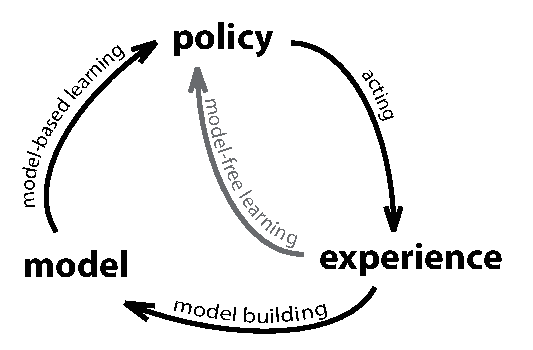
\includegraphics[width=.5\textwidth]{img/LearningPlanningActing}
	\caption[Dyna framework]{Integrating learning, planning and acting in the Dyna framework.}
	\label{fig:RL-integratingLearningPlanningActing}
\end{figure}

Dyna is the general term that is used for a class of algorithms that combine learning from real experiences with learning from simulated experiences generated using a (learned) model. We use the general term 'experience' to refer to a $(s,a,s',r)$-sample, which can be either obtained from observing the real system or by using the model. Various Dyna methods differ in the algorithms and the type of value function that are used. For example, Sutton introduces Dyna-Q and Dyna-PI that use Q-learning and Policy Iteration as learning algorithms respectively.

In a Dyna setting, every sampling interval starts with interaction with the real system. The observed state-transition and the resulting reward are used to update the value function and to update the model. Thereafter, a number of state-transitions are generated using the model. In short, the agent interacts with the system and the learned model alternatively (\figref{fig:RL-DynaFramework}).

The number of model-generated state-transitions can be either fixed or variable depending on the problem. In a real-time experiment for instance, the sampling interval can be used for model-based learning as long as there is time left. The ratio between real world and simulated samples can therefore vary. Algorithm \ref{alg:Dyna} shows Dyna-style learning in pseudo-code. The number of model-generated state-transitions every time step is fixed to \lsymb{$N_m$}{Number of model-generated state-transitions per time step}. Notice that the first part of the algorithms is on-line learning (identical to model-free SARSA learning), while the second part is off-line learning (based on the model). We have not explicitly indicated the building of the model in the algorithm. Depending on the implementation this could happen after every time step or episode.

\begin{figure}[htbp]
	\centering
		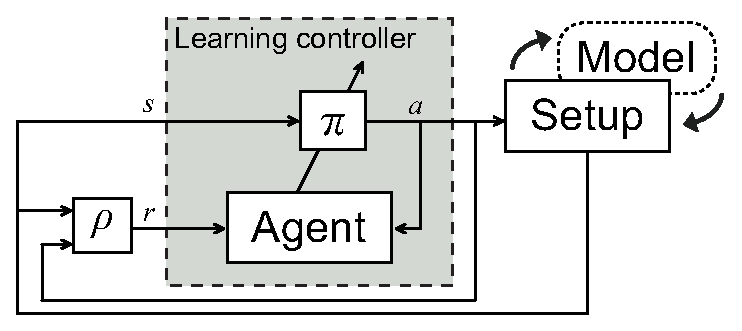
\includegraphics[width=.5\textwidth]{img/DynaFramework}
	\caption[Overview of the Dyna algorithm]{Schematic overview of the Dyna algorithm, which switches between interaction with the real system and its model.}
	\label{fig:RL-DynaFramework}
\end{figure}

\begin{algorithm}[ht]
	\caption{Dyna} \label{alg:Dyna}
	\begin{algorithmic}[1]
		\State Initialize $Q(s,a)$ randomly
		\For{ each time step $t$}
			\State $s\gets \textrm{ Current state}$
			\State Select $a$ using policy
			\State Execute $a$ and observe $s'$, $r$
			\State $\delta \gets r + \gamma Q(s',a') - Q(s,a)$
			\State $Q(s,a) \gets Q(s,a) + \alpha \delta$
			\Loop{ $N_m$ times}
				\State Select $(s,a)$ randomly
				\State $(s',r) \gets Model(s,a)$
				\State $\delta \gets r + \gamma Q(s',a') - Q(s,a)$
				\State $Q(s,a) \gets Q(s,a) + \alpha \delta$
			\EndLoop
		\EndFor
	\end{algorithmic}
\end{algorithm}

There is no restriction in the Dyna algorithm on the type of model that can be used. Also the needed accuracy of the model is not discussed in the literature. A general statement about the model can be made: the accuracy of the model should be high enough so that the model-based updates do not disturb the learning process. This statement is also true for real experiences, which can be noisy or disturbed measurements. The optimal ratio of real experience versus modeled experience might vary during the learning process. Early in the learning experiment, the model might still be inaccurate due to the low number of experiences. However, when the accuracy of the model increases, model-generated experiences might be a better representation of the true system than noisy measurements in the case of a deterministic system. Furthermore, the model might not have to be accurate in the entire state-space. The agent might also be able to find the goal if it  has an accurate model along trajectories directed towards the goal only.

%To have the most profit of using a model, it is important that the model is a good approximation of the real system. The model has to be accurate for the total state-space. \cite{Schmidhuber:91} introduces so-called curious model-building systems that include a confidence measure. Schmidhuber introduces the terms 'curiosity' and 'boredom' for part of the state-space that need to be visited or are already modeled accurately.
%	
%A variation on Dyna is \emph{experience replay} \cite{Lin:92}. Instead of learning a model, past transitions are simply stored. These past experiences are then used repeatedly by the algorithm.
	
The Dyna algorithm does not include a description of how to select the states that are updated in the planning. Is is generally assumed that the states are chosen randomly. However, this seems not to be the best choice for at least two reasons. Early in the learning process, most states will not contain any information regarding the goal state. The state's value will still be zero because the goal has never been reached from that state. Using these states in the planning will not lead to a useful value function update. Furthermore, in very large state-action spaces, not all states will be equally important for solving the learning problem. Only along trajectories towards the goal a good policy is required.

For these two reasons, it makes sense to concentrate the computational effort to areas of the state-action space where it is most effective. In other words, we want to prioritize important states in some way. A method that was introduced to update more important states first, is introduced next.

\subsubsection{Prioritized Sweeping}\label{sec:RL-Prioritized_sweeping}
	
Moore \cite{MooreAtkeson:93} and Peng \cite{PengWilliams:93} independently developed strategies to speed up the planning in Dyna by introducing a priority queue. Moore focused mainly on explicitly learning the state-transition model with all its transition probabilities. They named their method \ac{PS}. Peng used Dyna-Q as learning algorithm, and also used a priority queue to speed up learning. They named their method \emph{Queue-Dyna}. In both approaches, a queue is maintained that determines the order in which states should be updated during planning. The two methods are almost identical. They only differ in which states they allow onto the priority queue. Where \ac{PS} allows all predecessors which have a predicted change on the queue, Queue-Dyna allows only states that have a change greater than some threshold value. As mentioned, these differences are small and probably only influence memory usage in practice, but not learning speed. 
	
The importance of a state that determines its place in the queue can be determined in several ways. The general way is to take the absolute value of the \acs{TD}-error $\delta_t$. The larger this error, the more the value for a certain state has changed and thus the more influence it has on the total value function. Algorithm \ref{alg:PS} shows the \ac{PS} algorithm. Notice that the algorithm consists of an on-line and off-line part, which is similar to the Dyna algorithm. An important step in the \ac{PS} algorithm is determining lead-in states (Algorithm \ref{alg:PS}, line \ref{alg:PS_DetermineLeadInStates}). Lead-in states are state-action pairs $(\bar{s},\bar{a})$ that lead to state $s$. It is unclear how these states should be determined. In the literature one simply assumes that the model can produce them. In Chapter \ref{chap:Prioritized Sweeping} we will describe our approach to this problem.
	

\begin{algorithm}[ht]
	\caption{Prioritized Sweeping} \label{alg:PS}
	\begin{algorithmic}[1]
		\State Initialize $Q(s,a)$ randomly and $Queue$ empty
		\For{ each time step $t$}
			\State $s\gets \textrm{ Current state}$
			\State Select $a$ using policy
			\State Execute $a$ and observe $s'$, $r$
			\State $\delta \gets r + \gamma Q(s',a') - Q(s,a)$
			\State $Q(s,a) \gets Q(s,a) + \alpha \delta$
			\State Insert $(s,a)$ into $Queue$ with priority $| \delta |$
			\Loop{ $N_m$ times}
				\State Select $(s,a)$ from $Queue$
					\For{ each lead-in state $(\bar{s},\bar{a})$}\label{alg:PS_DetermineLeadInStates}
						\State $\delta \gets r + \gamma Q(s,a) - Q(\bar{s},\bar{a})$
						\State $Q(\bar{s},\bar{a}) \gets Q(\bar{s},\bar{a}) + \alpha \delta$
						\State Insert $(\bar{s},\bar{a})$ into $Queue$ with priority $| \delta |$
					\EndFor
			\EndLoop
		\EndFor
	\end{algorithmic}
\end{algorithm}

Most of the articles dealing with \ac{PS} techniques report improved learning speed compared to standard Dyna \cite{MooreAtkeson:93}, \cite{PengWilliams:93}, \cite{Rayner:07}, and also \cite{Wingate:05}. However, it has been reported that \ac{PS} can also lead to sub-optimal solutions for some specific tasks. For example \cite{Grzes:08} introduces a navigation task with one goal and several sub-goals. Using \ac{PS} in this task resulted in finding a sub-optimal solution. Grze\'{s} argues that this effect is due to the many sub-optimal solutions for the task. \ac{PS} would lead to insufficient exploration in such cases. However, it is not clear how the type of exploration, the exploration rate and learning rate influence this effect. 

%\section{Convergence properties}\label{sec:RL-Model_free_convergence_properties}
%So far we have not addressed the question whether or not the mentioned solution methods indeed lead to the optimal policy. This is the problem of convergence (to the optimal solution). Although this question is of great importance in RL (as it determines whether or not a solution will eventually be found), it is surprisingly often neglected. The majority of RL literature introduces new (variants of) algorithms and only heuristically shows their validity (i.e. by executing some learning experiment).
%
%We will not address convergence explicitly in this thesis. However, one important remark on the subject of convergence has to be made, which is valid for all solution methods. Since RL is essentially a trial-and-error method, the agent can only learn by visiting the entire state-action space. In fact, all state-action pairs would have to be visited continuously in order to guarantee convergence. This emphasises the importance of exploration. The algorithm has to continuously explore actions that do not seem optimal at that moment in the learning process. Furthermore, it also indicates that the complexity of a learning problem greatly increases with the number of state-action pairs as all the pairs have to be visited. 
%
%It is easy to see that a model-based methods will convergence, since it continuously visits all state-action pairs. Model-free methods also converge when all state-action pairs are visited. But this might be more difficult, because some states will only be visited very rarely. 



\section{Conclusions \& research opportunities}\label{sec:RL-Conclusions}
In this chapter, three different types of solution methods to the \acl{RL} problem were presented. Model-based methods use an available model of the environment to iteratively calculate the optimal value function. Model-free methods are used in an on-line setting where no explicit model of the environment is available. A combination of these two leads to Dyna-style methods in which model-free and model-based learning techniques are combined. \acl{PS} is an improvement of Dyna, as states are no longer updated randomly, but according to some priority measure.

%Different reasons were presented why model-learning techniques can improve learning speed compared to model-free methods. 

As described in Chapter \ref{chap:Introduction}, many interesting systems do not have an explicit model available. Therefore, purely model-based methods are of limited use in practical applications. On the other hand, purely model-free methods need long learning times because they can only interact with the real system once in every time interval. Therefore, model-learning methods seem to be the most promising method for the applications we consider in this work. The question how to build a model during learning is investigated further in Chapter \ref{chap:Modeling}. In order to have the most profit of the learned model, \ac{PS} seems to be an interesting technique to research. However, this technique has never been used on problems with a continuous state-space. The implementation of the model and \ac{PS} in the learning algorithms are described in Chapter \ref{chap:Prioritized Sweeping}.

